\section{Pure Cross-sectional Analysis}

\begin{frame}{Model Setup - True DGP}

\Large
\[y_i = \beta_1 x_{1i} + \beta_2 x_{2i} + \epsilon_i, \ \ \epsilon_i \stackrel{i.i.d}{\sim} N(0,\sigma^2_{\epsilon})\]

\vspace{5mm}
\normalsize
\begin{itemize}
    \item $E[x_{1i}] = E[x_{2i}] = 0$, $Var(x_{1i}) = Var(x_{2i}) = 1$
    \item $Cov(x_{1i}, x_{2i}) = 0.3$ exogenous and weakly correlated regressors
    \item $\pmb{\beta} = (\beta_1, \beta_2)' = (2,2)'$, $\sigma^2_{\epsilon}=4$
    \item All classical assumptions
    \vspace{3mm}
    \item Obtain $y$, $x_{1i}$ and $x_{2i}$
\end{itemize}

\end{frame}



\begin{frame}{Model Setup - Forecasting Models}

The constituent models in matrix form are proposed as
\Large
\begin{align*}
M_1 : y &= x_1 \alpha_{1} + u_1, \ \ u_{1} \stackrel{i.i.d}{\sim} N(0,\sigma^2_1) \\
M_2 : y &= x_2 \alpha_{2} + u_2, \ \ u_{2} \stackrel{i.i.d}{\sim} N(0,\sigma^2_2).
\end{align*}
\normalsize
\begin{itemize}
    \item Obtain $\hat y_{1}$ from $M_1$ and $\hat y_{2}$ from $M_2$
    \vspace{3mm}
    \item Aggregate them linearly $\hat y = \hat y_{1}\omega + \hat y_{2}(1-\omega)$
\end{itemize}

\end{frame}



\begin{frame}{Optimal Weight Derivation - Minimization}

The optimal weight is obtained over the in-sample period (R).
\vspace{-1mm}
\begin{align*}
\hat{\omega}_{\text{opt}} 
&= \underset{\omega \in [0,1]}{\arg\min} \ \frac{1}{R} \sum^R_{t=1} \Big[y - \big(\hat y_{1} \omega + \hat y_{2} (1-\omega)\big)\Big]' \Big[y - \big(\hat y_{1} \omega + \hat y_{2} (1-\omega)\big)\Big] \\
&= \underset{\omega \in [0,1]}{\arg\min} \ \frac{1}{R} \sum^R_{t=1} \Big[y - \big(x_1 \hat\alpha_1 \omega + \ x_2 \hat\alpha_2 (1-\omega)\big)\Big]'\Big[y - \big(x_1 \hat\alpha_1 \omega + \ x_2 \hat\alpha_2 (1-\omega)\big)\Big] \\
&= \underset{\omega \in [0,1]}{\arg\min} \ \frac{1}{R} \sum^R_{t=1} \big[y-(x_1 \hat\alpha_1 - x_2 \hat\alpha_2) \omega - x_2 \hat\alpha_2\big]'\big[y-(x_1 \hat\alpha_1 - x_2 \hat\alpha_2) \omega - x_2 \hat\alpha_2\big]
\end{align*}

\onslide<2-> \[-2(x_1 \hat\alpha_1 - x_2 \hat\alpha_2)' (y-(x_1 \hat\alpha_1 - x_2 \hat\alpha_2) \hat\omega_{opt} - x_2 \hat\alpha_2) = 0\]

\end{frame}



\begin{frame}{Optimal Weight Derivation - Findings}

\begin{align*}
\hat\omega_{opt} 
&= \frac{(x_1 \hat\alpha_1 - x_2 \hat\alpha_2)' y - (x_1 \hat\alpha_1 - x_2 \hat\alpha_2)' x_2 \hat\alpha_2}{\hat\alpha'_1 x'_1 x_1 \hat\alpha_1 - 2\hat\alpha'_1 x'_1 x_2 \hat\alpha_2 + \hat\alpha'_2 x'_2 x_2 \hat\alpha_2} \\
&= \frac{\alt<1>{\alert{\hat\alpha_1'}}{\hat\alpha_1'}\alt<2>{\alert{\text{cov}_R(x_1,x_1)}}{\text{cov}_R(x_1,x_1)}\alt<1>{\alert{\hat\alpha_1}}{\hat\alpha_1} - \alt<1>{\alert{\hat\alpha_1'}}{\hat\alpha_1'}\alt<3>{\alert{\text{cov}_R(x_1,x_2)}}{\text{cov}_R(x_1,x_2)}\alt<1>{\alert{\hat\alpha_2}}{\hat\alpha_2}}{\alt<1>{\alert{\hat\alpha_1'}}{\hat\alpha_1'} \alt<2>{\alert{\text{cov}_R(x_1,x_1)}}{\text{cov}_R(x_1,x_1)}\alt<1>{\alert{\hat\alpha_1}}{\hat\alpha_1} - 2\alt<1>{\alert{\hat\alpha_1'}}{\hat\alpha_1'}\alt<3>{\alert{\text{cov}_R(x_1,x_2)}}{\text{cov}_R(x_1,x_2)}\alt<1>{\alert{\hat\alpha_2}}{\hat\alpha_2} + \alt<1>{\alert{\hat\alpha_2'}}{\hat\alpha_2'}\alt<2>{\alert{\text{cov}_R(x_1,x_1)}}{\text{cov}_R(x_2,x_2)}\alt<1>{\alert{\hat\alpha_2}}{\hat\alpha_2}}
\end{align*}

\vspace{3mm}

The estimated optimal weight $\hat\omega_{opt}$ is affected by
    \begin{enumerate}[<+->]
        \item the magnitude of estimated coefficient(s) in each constituent model 
        \item the variances of regressors
        \item the covariance of regressors 
    \end{enumerate}

\end{frame}



\begin{frame}{Optimal Weight Derivation - Limiting Result}
\[\hat\omega_{opt} \overset{p}{\to} \omega_\star 
    = \frac{\alpha_1'\Sigma_{11}\alpha_1 - \alpha_1'\Sigma_{12}\alpha_2}{\alpha_1'\Sigma_{11}\alpha_1 - 2\alpha_1'\Sigma_{12}\alpha_2 + \alpha_2'\Sigma_{22}\alpha_2}\]

\vspace{3mm}

For $\omega_\star = \frac{1}{2}$, it must be that 
\[\alpha_1'\Sigma_{11}\alpha_1 = \alpha_2'\Sigma_{22}\alpha_2.\]

\vspace{3mm}

Asymptotically, any situation where this final equality is nearly satisfied will inevitably lead the optimal weight to be around a half.
\end{frame}



\begin{frame}[plain]
    \begin{figure}
        \centering
        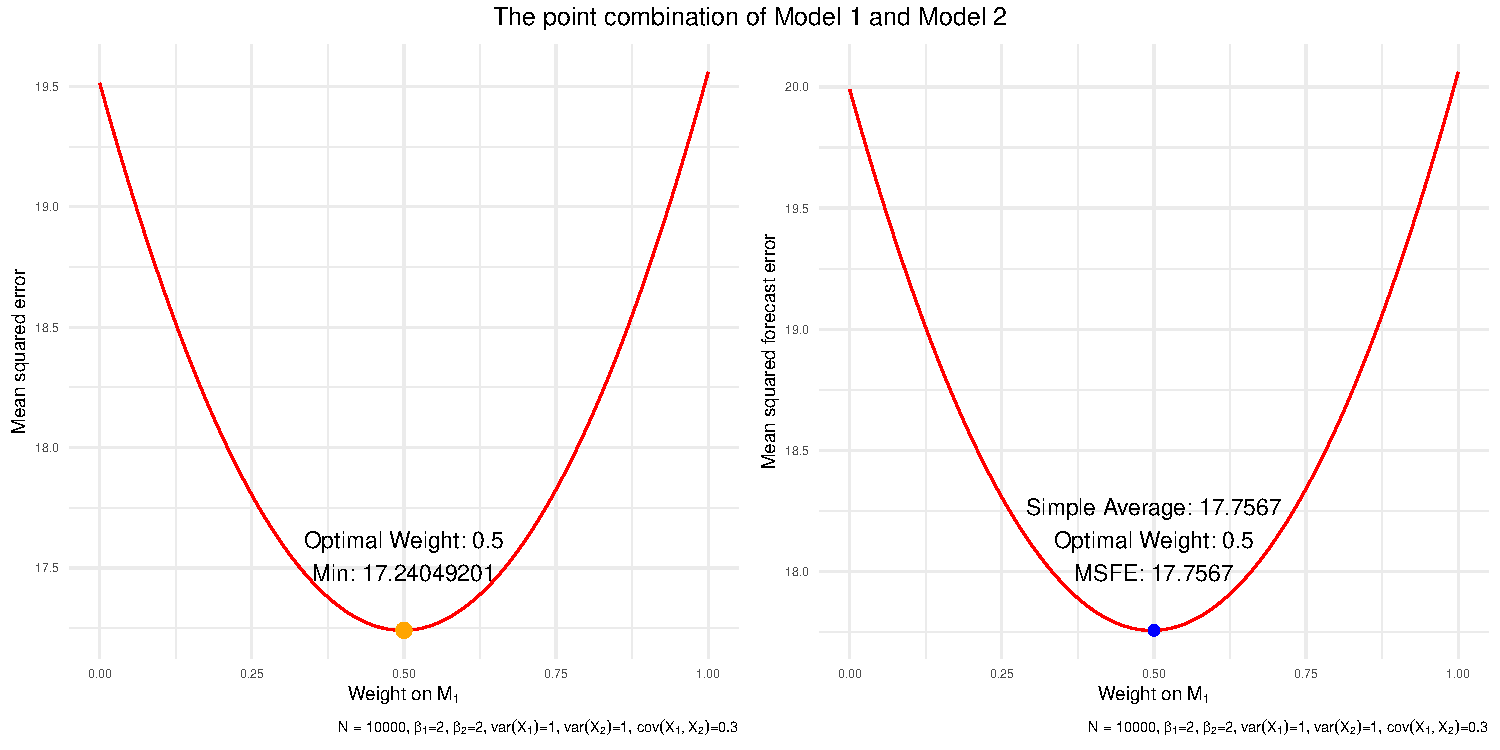
\includegraphics[scale=0.55]{Graph/MSFE.pdf}
        \caption{\footnotesize{$\hat\omega_{opt}$ = 0.5, \alert{N = 10000}, $\beta_1$=2, $\beta_2$=2, $var(X_1)$=1, $var(X_2)$=1, $cov(X_1,X_2)$=0.3}}
    \end{figure}
\end{frame}



\begin{frame}{Density Simulations}
    Applying the learning to density combinations 
    
    \begin{itemize}
        \item Log scoring rules
        \item No closed-form expression
        \item Applicability of findings
    \end{itemize}

\end{frame}



\begin{frame}[plain]
    \begin{figure}
        \centering
        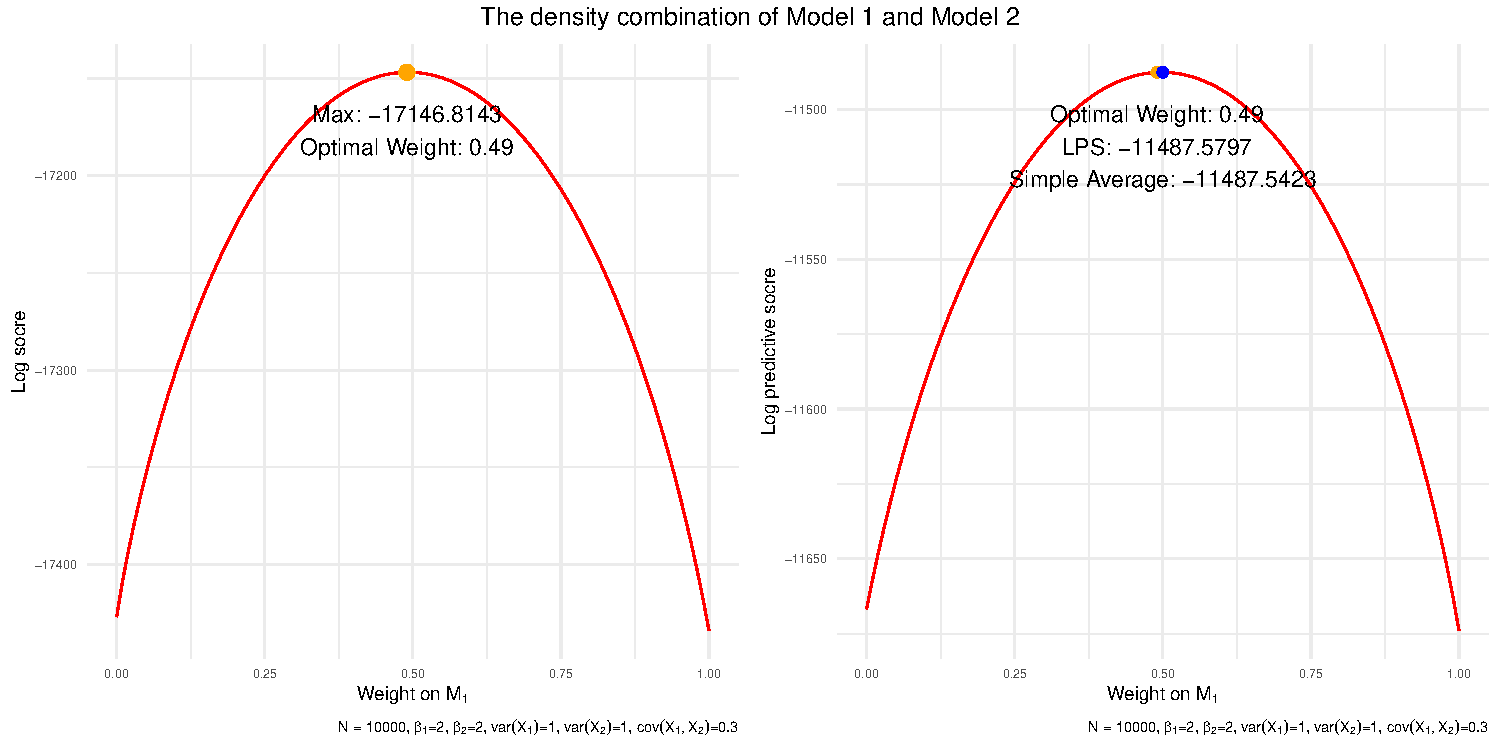
\includegraphics[scale=0.55]{Graph/LPS_10000.pdf}
        \caption{\footnotesize{$\hat\omega_{opt}$ = 0.49, N = 10000, $\beta_1$=2, $\beta_2$=2, $var(X_1)$=1, $var(X_2)$=1, $cov(X_1,X_2)$=0.3}}
    \end{figure}
\end{frame}



\begin{frame}[plain]
    \begin{figure}
        \centering
        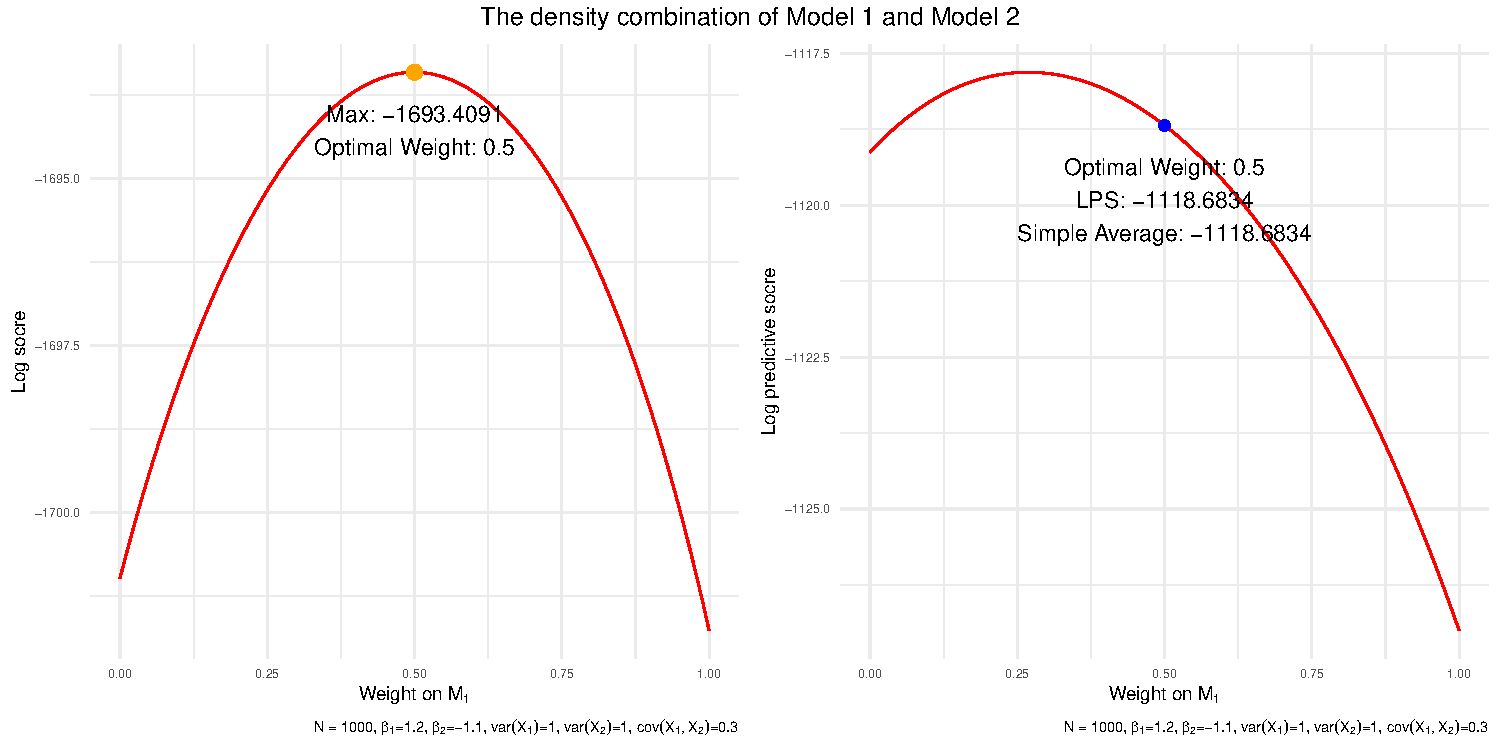
\includegraphics[scale=0.55]{Graph/LPS_1000.pdf}
        \caption{\footnotesize{\alert{$\hat\omega_{opt}$ = 0.5}, N = 1000, \alert{$\beta_1$=1.2}, \alert{$\beta_2$=-1.1}, $var(X_1)$=1, $var(X_2)$=1, $cov(X_1,X_2)$=0.3}}
    \end{figure}
\end{frame}



\begin{frame}[plain]
    \begin{figure}
        \centering
        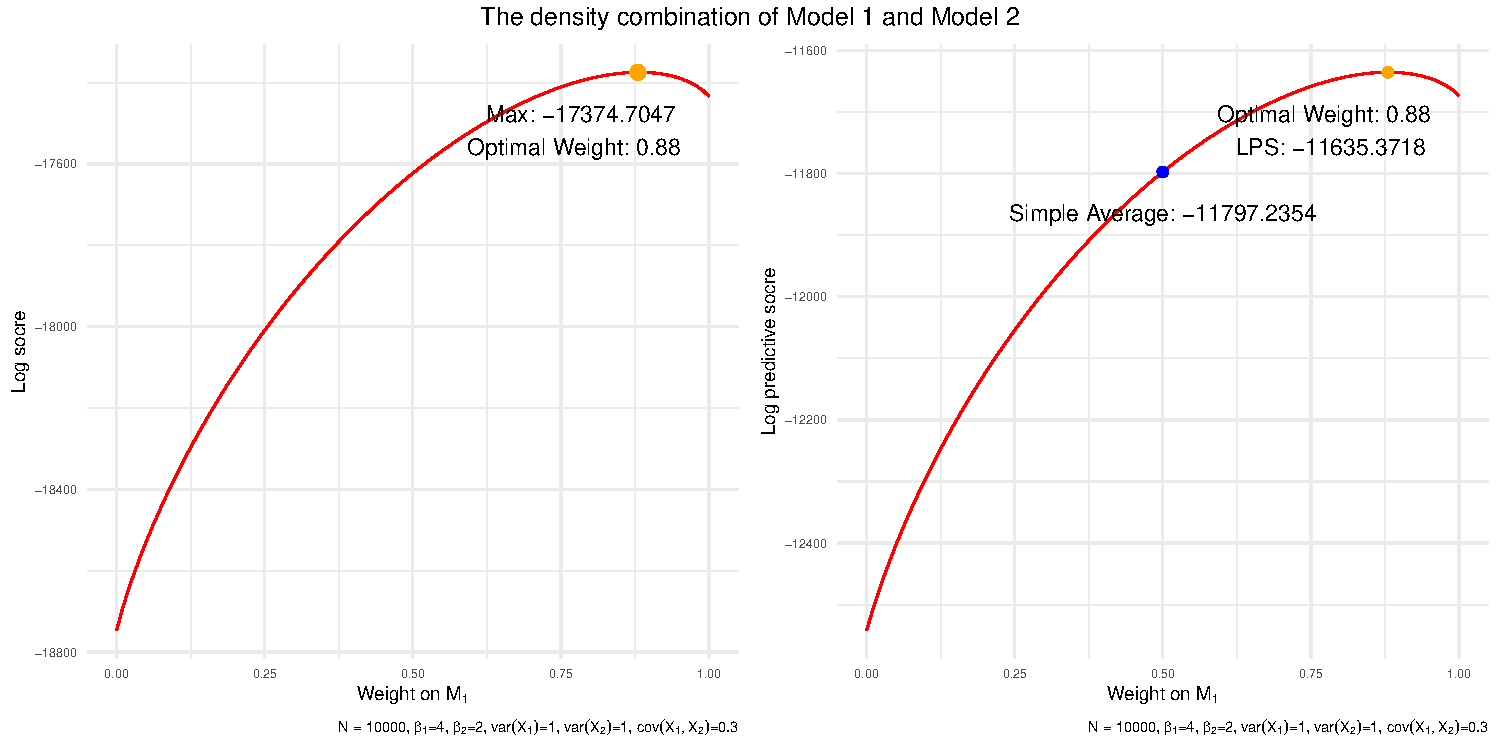
\includegraphics[scale=0.55]{Graph/LPS_1.pdf}
        \caption{\footnotesize{\alert{$\hat\omega_{opt}$ = 0.88}, N = 10000, \alert{$\beta_1$=4}, \alert{$\beta_2$=2}, $var(X_1)$=1, $var(X_2)$=1, $cov(X_1,X_2)$=0.3}}
    \end{figure}
\end{frame}



\begin{frame}[plain]
    \begin{figure}
        \centering
        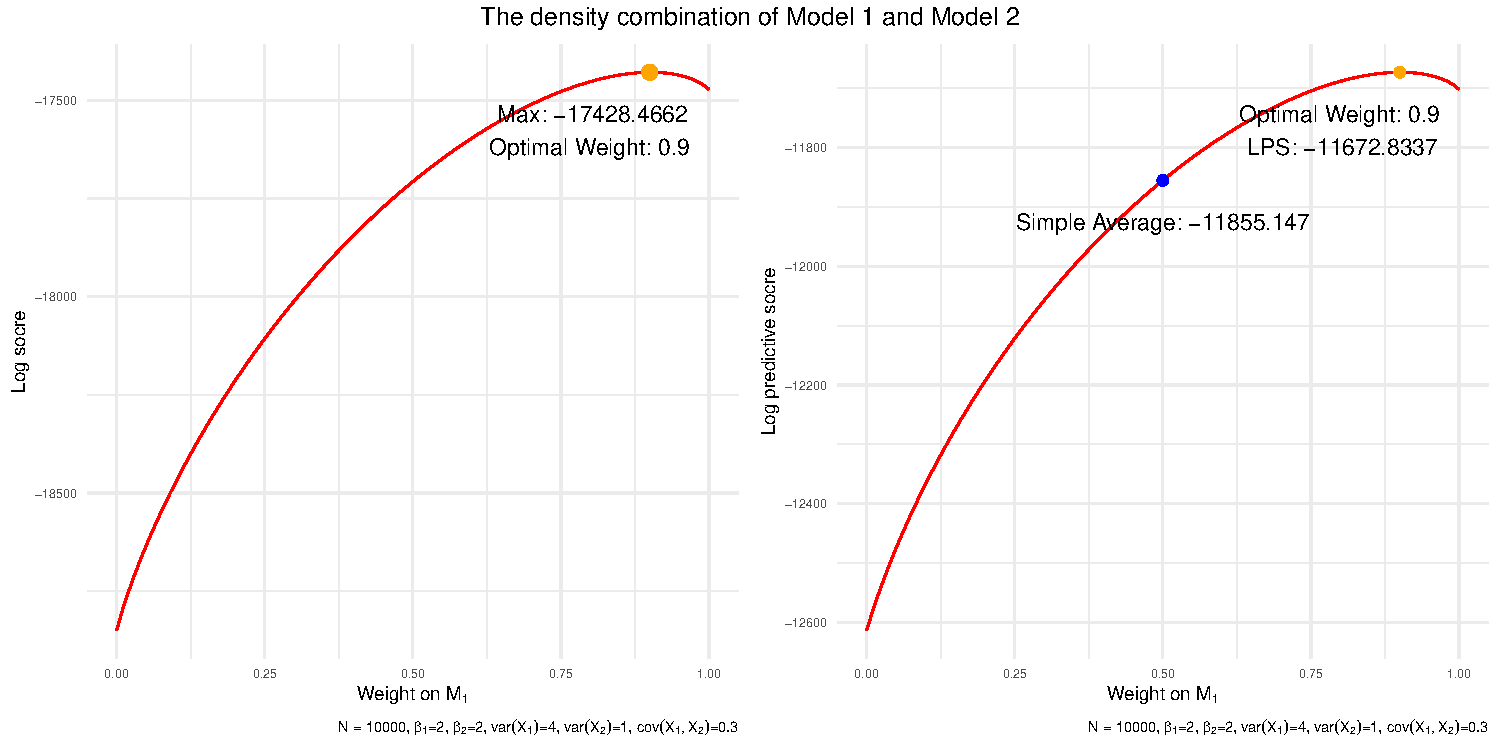
\includegraphics[scale=0.55]{Graph/LPS_2.pdf}
        \caption{\footnotesize{\alert{$\hat\omega_{opt}$ = 0.9}, N = 10000, $\beta_1$=2, $\beta_2$=2, \alert{$var(X_1)$=4}, \alert{$var(X_2)$=1}, $cov(X_1,X_2)$=0.3}}
    \end{figure}
\end{frame}





